\documentclass[aspectratio=169,14pt,fleqn]{beamer}
\usetheme{Madrid}
\usecolortheme{dolphin}
\setbeamertemplate{navigation symbols}{}
\usepackage[utf8]{inputenc}
\usepackage[T1]{fontenc}
\usepackage{graphicx}
\usepackage[table]{xcolor}
\usepackage{microtype}
\usepackage{amsmath,amssymb,array}
\usepackage{tikz}
\usetikzlibrary{positioning,decorations.pathmorphing}
\usetikzlibrary{calc}




\title{Week 3}
\author{Hans Halvorson}
\date{September 22, 2025}

\AtBeginSection[]{
  \begin{frame}
    \centering
    \vfill
    \Huge\insertsectionhead
    \vfill
  \end{frame}
}

\begin{document}

\frame{\titlepage}

\section{Reductio ad Absurdum}

% --- Intro ---
\begin{frame}{Introduction}
 
  \begin{itemize}
  \item Idea behind Reductio ad Absurdum: Show that something is
    \textbf{not} the case ($\neg A$) by showing that it ($A$) leads,
    via logically valid reasoning, to a contradiction.
  \begin{itemize}
  \item RA is truly powerful if combined with DN-elimination to
    establish \textbf{positive} conclusions.
  \end{itemize}
  \end{itemize}
  
\end{frame}

\begin{frame}{$\sqrt{2}$ is not a rational number}

\small 
\medskip \textbf{Proof.} Assume for reductio ad absurdum that
$\sqrt{2}$ is rational, i.e.\ that \(\sqrt{2}=\dfrac{a}{b}\) with
integers \(a,b\) in lowest terms (\(\gcd(a,b)=1\), \(b\neq 0\)).  Then
\[
  2=\frac{a^2}{b^2}\;\Rightarrow\; a^2=2b^2.
\]
Hence \(a^2\) is even, so \(a\) is even; write \(a=2k\).
Substituting,
\[
(2k)^2=2b^2 \;\Rightarrow\; 4k^2=2b^2 \;\Rightarrow\; b^2=2k^2,
\]
so \(b^2\) is even and therefore \(b\) is even.

\medskip Thus both \(a\) and \(b\) are even, contradicting that
\(\frac{a}{b}\) is in lowest terms. Therefore, \(\sqrt{2}\) is
irrational. \(\square\)
\end{frame}


\begin{frame}{Reductio ad Absurdum}

  
  \bigskip
  \begin{tabular}{>{\raggedleft\arraybackslash}p{4cm}
      >{\centering\arraybackslash}p{1.0cm} p{5cm}
      >{\raggedright\arraybackslash}p{3.5cm}}
    $m$ & ($m$) & $A$ & A \\
        & \,\vdots & \\
    $n_1,\dots ,n_j$ & ($n$) & $B\wedge\neg B$ & \\
        & \,\vdots & \\
    $n_1,\ldots,\widehat{m},\ldots,n_j$ & ($k$) & $\neg A$ &
                                                             $m,n$ RA \end{tabular}
\end{frame}

\begin{frame}{Reductio ad Absurdum}
  \centering
  \scalebox{1.3}{%
    \colorbox{yellow!20}{%
      $\begin{array}{c}
         A_1,\dots ,A_n,B \: \vdash \: \bot \\[6pt] \hline \\[-6pt]
         A_1,\dots ,A_n \: \vdash \: \neg B
       \end{array}$%
    }%
  }
\end{frame}

\begin{frame}
  \bigskip

\begin{tabular}{>{\raggedleft\arraybackslash}p{1.5cm} >{\centering\arraybackslash}p{1.0cm} p{5cm} >{\raggedright\arraybackslash}p{3.5cm}}
1 & (1) & $\neg \mathit{P} \to \mathit{P}$ & A \\
2 & (2) & $\neg \mathit{P}$ & A \\
1,2 & (3) & $\mathit{P}$ & 1,2 MP \\
1,2 & (4) & $\mathit{P} \wedge \neg \mathit{P}$ & 3,2 $\wedge$I \\
1 & (5) & $\neg \neg \mathit{P}$ & 2,4 RA \\
1 & (6) & $\mathit{P}$ & 5 DN \\
\end{tabular}

\end{frame}



% --- DeMorgan's 1 ---
\begin{frame}{DeMorgan's laws}

Show $\neg (P\vee Q)\vdash \neg P$

\bigskip \begin{tabular}{>{\raggedleft\arraybackslash}p{1.5cm}
                >{\centering\arraybackslash}p{1.0cm}
                p{5cm}
                >{\raggedright\arraybackslash}p{3.5cm}}
1 & (1) & $\neg(P\vee Q)$ & A \\
2 & (2) & $P$ & A \\
2 & (3) & $P\vee Q$ & 2 $\vee$I \\
1,2 & (4) & $(P\vee Q)\wedge\neg(P\vee Q)$ & 3,1 $\wedge$I \\
1 & (5) & $\neg P$ & 2,4 RA \\
\end{tabular}

\end{frame}

\begin{frame}{Material conditional}
Show $\neg(\neg P\vee Q)\vdash \neg(P\to Q)$

\bigskip
\begin{tabular}{>{\raggedleft\arraybackslash}p{1.5cm}
                >{\centering\arraybackslash}p{1.0cm}
                p{5cm}
                >{\raggedright\arraybackslash}p{4cm}}
1 & (1) & $\neg(\neg P\vee Q)$ & A \\
2 & (2) & $P\to Q$ & A \\
1 & (3) & $\neg\neg P$ & see previous proof \\
1 & (4) & $P$ & 3 DN \\
1,2 & (5) & $Q$ & 2,4 MP \\
1,2 & (6) & $\neg P\vee Q$ & 5 $\vee$I \\
1,2 & (7) & $(\neg P\vee Q)\wedge\neg(\neg P\vee Q)$ & 6,1 $\wedge$I \\
1 & (8) & $\neg(P\to Q)$ & 2,7 RA \\
\end{tabular}

\end{frame}

% --- Non-Contradiction ---
\begin{frame}{Law of Non-Contradiction}

\bigskip 
\begin{tabular}{>{\raggedleft\arraybackslash}p{1.5cm}
                >{\centering\arraybackslash}p{1.0cm}
                p{5cm}
                >{\raggedright\arraybackslash}p{3.5cm}}
1 & (1) & $P\wedge \neg P$ & A \\
  & (2) & $\neg(P\wedge \neg P)$ & 1,1 RA \\
\end{tabular}
\end{frame}



% --- EFQ ---
\begin{frame}{Ex Falso Quodlibet (EFQ)}

\bigskip \begin{tabular}{>{\raggedleft\arraybackslash}p{1.5cm}
                >{\centering\arraybackslash}p{1.0cm}
                p{5cm}
                >{\raggedright\arraybackslash}p{3.5cm}}
1 & (1) & $P$ & A \\
2 & (2) & $\neg P$ & A \\
3 & (3) & $\neg Q$ & A \\
1,2 & (4) & $P\wedge \neg P$ & 1,2 $\wedge$I \\
1,2 & (5) & $\neg\neg Q$ & 3,4 RA \\
1,2 & (6) & $Q$ & 5 DN \\
         \end{tabular}

         \bigskip It is \textbf{not} required that the assumption
         occurs in the dependencies of the contradiction.

\end{frame}

% --- DS ---
\begin{frame}{Disjunctive Syllogism}

  $P\vee Q, \neg P\:\vdash \:Q$

\bigskip \begin{tabular}{>{\raggedleft\arraybackslash}p{1.5cm}
                >{\centering\arraybackslash}p{1.0cm}
                p{5cm}
                >{\raggedright\arraybackslash}p{3.5cm}}
1 & (1) & $P\vee Q$ & A \\
2 & (2) & $\neg P$ & A \\
3 & (3) & $P$ & A \\
2,3 & (4) & $Q$ & EFQ \\
5 & (5) & $Q$ & A \\
1,2 & (6) & $Q$ & 1,3,4,5,5 $\vee$E \\
\end{tabular}

\end{frame}

% --- DeMorgan's III ---
\begin{frame}{DeMorgan's Laws}
$\neg P\vee \neg Q\:\vdash\:\neg(P\wedge Q)$

\bigskip 
\begin{tabular}{>{\raggedleft\arraybackslash}p{1.5cm}
                >{\centering\arraybackslash}p{1.0cm}
                p{5cm}
                >{\raggedright\arraybackslash}p{3.5cm}}
1 & (1) & $\neg P$ & A \\
2 & (2) & $P\wedge Q$ & A \\
2 & (3) & $P$ & 2 $\wedge$E \\
1,2 & (4) & $P\wedge \neg P$ & 3,1 $\wedge$I \\
1 & (5) & $\neg(P\wedge Q)$ & 2,4 RA \\
\end{tabular}

\end{frame}

\begin{frame}{DeMorgan's Laws}
  $\neg P,\neg Q \:\vdash \:\neg(P\vee Q)$

  \bigskip By DS we have $\neg P,P\vee Q\vdash Q$.

  \medskip It follows that $\neg P,P\vee Q,\neg Q\vdash\bot$.

  \medskip By RA, $\neg P,\neg Q\vdash \neg (P\vee Q)$.

\end{frame}

\begin{frame}  

\bigskip {\begin{tabular}{>{\raggedleft\arraybackslash}p{1.5cm}
                >{\centering\arraybackslash}p{1.0cm}
                p{5cm}
                >{\raggedright\arraybackslash}p{3.5cm}}
1 & (1) & $P\vee Q$ & A \\
2 & (2) & $\neg P$ & A \\
3 & (3) & $P$ & A \\
4 & (4) & $\neg Q$ & A \\
2,3 & (5) & $P\wedge \neg P$ & 3,2 $\wedge$I \\
2,3 & (6) & $\neg\neg Q$ & 4,5 RA \\
2,3 & (7) & $Q$ & 6 DN \\
8 & (8) & $Q$ & A \\
1,2 & (9) & $Q$ & 1,3,7,8,8 $\vee$E \\
1,2,4 & (10) & $Q\wedge \neg Q$ & 9,4 $\wedge$I \\
2,4 & (11) & $\neg(P\vee Q)$ & 1,10 RA \\
                 \end{tabular}
                 }

               \end{frame}

% --- Excluded Middle ---
\begin{frame}{Law of Excluded Middle}

\begin{tabular}{>{\raggedleft\arraybackslash}p{1.5cm}
                >{\centering\arraybackslash}p{1.0cm}
                p{5cm}
                >{\raggedright\arraybackslash}p{3.5cm}}
1 & (1) & $\neg(P\vee \neg P)$ & A \\
2 & (2) & $P$ & A \\
2 & (3) & $P\vee \neg P$ & 2 $\vee$I \\
1,2 & (4) & $(P\vee \neg P)\wedge\neg(P\vee \neg P)$ & 3,1 $\wedge$I \\
1 & (5) & $\neg P$ & 2,4 RA \\
1 & (6) & $P\vee \neg P$ & 5 $\vee$I \\
1 & (7) & $(P\vee \neg P)\wedge\neg(P\vee \neg P)$ & 6,1 $\wedge$I \\
  & (8) & $\neg\neg(P\vee \neg P)$ & 1,7 RA \\
  & (9) & $P\vee \neg P$ & 8 DN \\
\end{tabular}
\end{frame}
               




\begin{frame}{More difficult proofs}
  To show: $P\to(Q\vee R)\:\vdash\: (P\to Q)\vee(P\to R)$

  \medskip \begin{itemize}
  \item Strategy 1: Assume negation of conclusion, apply
    DeMorgans. The result is two negated conditionals, which are
    equivalent to conjunctions.
\item Strategy 2: Derive $P\vee\neg P$, then argue by cases. Recall
  that $\neg P\vdash P\to Q$.
\end{itemize}
\end{frame}

\begin{frame}{Useful sequents}

\newcommand{\id}{\:\dashv\vdash\:}

\begin{block}{}
\begin{tabular}{>{\bfseries}l l}
Commutativity: & $A \wedge B \id B \wedge A$ \\
               & $A \vee B \id B \vee A$ \\[6pt]

Associativity: & $(A \wedge B)\wedge C \id A \wedge (B \wedge C)$ \\
               & $(A \vee B)\vee C \id A \vee (B \vee C)$ \\[6pt]

Distributivity: & $A \wedge (B \vee C) \id (A \wedge B)\vee (A \wedge C)$ \\
                & $A \vee (B \wedge C) \id (A \vee B)\wedge (A \vee C)$ \\[6pt]

De Morgan’s I: & $\neg (A \vee B) \id \neg A \wedge \neg B$ \\
               & $\neg (A \wedge B) \id \neg A \vee \neg B$ \\
\end{tabular}
\end{block}

\end{frame}

\begin{frame}{Useful sequents}

\newcommand{\id}{\:\dashv\vdash\:}

\begin{block}{}
\begin{tabular}{>{\bfseries}l l}
  Material Conditional: & $A \to B \id \neg A \vee B$ \\
  & $\neg (A\to B) \id A\wedge \neg B$ \\[6pt]

Excluded Middle:      & $\vdash \;A \vee \neg A$ \\[6pt]

Disjunctive Syllogism: & $A \vee B, \;\neg A \;\vdash\; B$ \\
\end{tabular}
\end{block}

\end{frame}




\section{Truth tables}

\begin{frame}{How do you know if something can be proven?}

  \begin{itemize}
  \item If you prove $A_1,\dots ,A_n\vdash B$, then that argument form
    is truth preserving (in the sense that we are about to make
    precise).
  \item If you fail to prove $A_1,\dots ,A_n\vdash B$, that doesn’t
    prove that it is not provable.
  \item If you can show that $A_1,\dots ,A_n\vdash B$ is not
    truth-preserving, then there cannot possibly be a proof of
    $A_1,\dots ,A_n\vdash B$.
  \end{itemize}

\end{frame}

\begin{frame}{Semantic validity}

  \begin{itemize}
  \item An argument form is \textbf{semantically invalid} if there is
    an instance of that form where the premises are true and the
    conclusion is false.
    \begin{itemize}
    \item A \textbf{counterexample} to the validity of an argument is
      an assignment of truth values to the atomic sentences that makes
      that argument's premises true and its conclusion false.
    \end{itemize}
  \item We write $A_1,\dots ,A_n\vDash B$ to indicate that the
    argument from $A_1,\dots ,A_n$ to $B$ is semantically valid.
  \end{itemize}

\end{frame}

\begin{frame}{Ways Things Could Be}
\centering
\begin{tabular}{c c c}
  $P$ & $Q$ & $R$ \\
  \hline
  1 & 1 & 1 \\
  1 & 1 & 0 \\
  1 & 0 & 1 \\
  1 & 0 & 0 \\
  0 & 1 & 1 \\
  0 & 1 & 0 \\
  0 & 0 & 1 \\
  0 & 0 & 0 \\
\end{tabular}
\end{frame}



% \begin{frame}{Scenarios, aka Ways Things Could Be}

% \begin{tabular}{ccc}
% $P$ & $Q$  & $R$  \\
% \hline
% \foreach \P in {1,0}{%
%   \foreach \Q in {1,0}{%
%     \foreach \R in {1,0}{%
%       \P & \Q & \R \\
% }}}
% \end{tabular}
% \end{frame}

\begin{frame}{Truth Tables}

\begin{columns}[t]

\column{0.48\textwidth}
\textbf{Conjunction $\wedge$}

{\footnotesize
\[
\begin{array}{c c | c}
P & Q & P \wedge Q \\
\hline
1 & 1 & 1 \\
1 & 0 & 0 \\
0 & 1 & 0 \\
0 & 0 & 0 \\
\end{array}
\]}

\medskip
\textbf{Disjunction $\vee$}

{\footnotesize
\[
\begin{array}{c c | c}
P & Q & P \vee Q \\
\hline
1 & 1 & 1 \\
1 & 0 & 1 \\
0 & 1 & 1 \\
0 & 0 & 0 \\
\end{array}
\]}

\column{0.48\textwidth}
\textbf{Negation $\neg$}

{\footnotesize
\[
\begin{array}{c | c}
P & \neg P \\
\hline
1 & 0 \\
0 & 1 \\
\end{array}
\]}

\medskip
\textbf{Conditional $\to$}

{\footnotesize
\[
\begin{array}{c c | c}
P & Q & P \to Q \\
\hline
1 & 1 & 1 \\
1 & 0 & 0 \\
0 & 1 & 1 \\
0 & 0 & 1 \\
\end{array}
\]}
\end{columns}

\end{frame}

\begin{frame}{Detailed truth table for $(P \wedge \neg Q) \to R$}

{\small
\[
\begin{array}{ccc|cccccccc}
P & Q & R & ( & P & \wedge & \neg & Q & ) & \to & R \\
\hline
1 & 1 & 1 & \phantom{0} & 1 & 0 & 0 & 1 & \phantom{0} & 1 & 1 \\
1 & 1 & 0 & \phantom{0} & 1 & 0 & 0 & 1 & \phantom{0} & 1 & 0 \\
1 & 0 & 1 & \phantom{0} & 1 & 1 & 1 & 0 & \phantom{0} & 1 & 1 \\
1 & 0 & 0 & \phantom{0} & 1 & 1 & 1 & 0 & \phantom{0} & \mathbf{\color{red}0} & 0 \\
0 & 1 & 1 & \phantom{0} & 0 & 0 & 0 & 1 & \phantom{0} & 1 & 1 \\
0 & 1 & 0 & \phantom{0} & 0 & 0 & 0 & 1 & \phantom{0} & 1 & 0 \\
0 & 0 & 1 & \phantom{0} & 0 & 0 & 1 & 0 & \phantom{0} & 1 & 1 \\
0 & 0 & 0 & \phantom{0} & 0 & 0 & 1 & 0 & \phantom{0} & 1 & 0 \\
\end{array}
\]
}

This sentence is a \textbf{contingency}: true in some scenarios and
false in other scenarios
\end{frame}

\begin{frame}{Material conditional}

{\centering\large 
\[
\begin{array}{c c | c}
P & Q & P \to Q \\
\hline
1 & 1 & 1 \\
1 & 0 & 0 \\
0 & 1 & 1 \\
0 & 0 & 1 \\
\end{array}
\]
}

\bigskip ``If the Germans won World War II then French is the official
language of instruction at Princeton.'' 

\end{frame}

\begin{frame}{Negative paradox is valid}

\[
\begin{array}{c c | c | c}
P & Q & \neg P & P \to Q \\
\hline
  1 & 1 &  0 & 1 \\
  1 & 0 &  0 & 0 \\
  0 & 1 & 1 & 1 \\ % <-- highlight whole row
  0 & 0 & 1 & 1 \\
\end{array}
\]

\medskip In every case where the premise $\neg P$ is true, the
conclusion $P\to Q$ is also true.

\end{frame}



\begin{frame}{Affirming the consequent is invalid}

  $P\to Q,Q\:\not\vDash\: P$

\[
\begin{array}{c c | c}
P & Q & P \to Q \\
\hline
  1 & 1 & 1 \\
  1 & 0 & 0 \\
\rowcolor{red!20} 0 & 1 & 1 \\ % <-- highlight whole row
0 & 0 & 1 \\
\end{array}
\]  

\medskip In row 3, both premises ($P \to Q$ and $Q$) are true, but the
conclusion $P$ is false. Therefore the argument form is
\textbf{invalid}.
\end{frame}



\begin{frame}{Ex Falso Quodlibet: $P, \neg P \;\therefore Q$}

\[
\begin{array}{c c | c | c | c}
P & Q & \neg P & \text{Premises all true?} & \text{Conclusion $Q$} \\
\hline
1 & 1 & 0 & \text{no} & 1 \\
1 & 0 & 0 & \text{no} & 0 \\
0 & 1 & 1 & \text{no} & 1 \\
0 & 0 & 1 & \text{no} & 0 \\
\end{array}
\]

\medskip
The premises $P$ and $\neg P$ can never both be true.  
So there is no row where all premises are true and the conclusion false.  
Hence the argument form is \textbf{valid}.
\end{frame}

\section{Using truth tables to guide proofs}

\begin{frame}

  Is there a correctly written proof with line fragments like this?

  \vspace{2em}
  \begin{tabular}{>{\raggedleft\arraybackslash}p{1.5cm}
                >{\centering\arraybackslash}p{1.0cm}
    p{4.5cm}
      >{\raggedright\arraybackslash}p{2cm}}
    1 & (1) & $P\vee Q$ & A \\
      & \,\vdots & \\
    1 & (n) & $P$ \end{tabular}

  \pause 

  \bigskip No there cannot be. Our proof rules are \textbf{sound}, so
  they cannot prove a line that is semantically invalid.

\end{frame}

\begin{frame}{Soundness}

  \textbf{Fact:} If there is a correctly written proof that ends with
  $A_1,\dots ,A_n\vdash B$, then $A_1,\dots ,A_n\vDash B$.

  \bigskip Consequently, if $A_1,\dots ,A_n\not\vDash B$, then there
  cannot be a correctly written proof that ends with
  $A_1,\dots ,A_n\vdash B$.

  \medskip In other words, if there is a \textbf{counterexample}, then
  there is no proof.



\end{frame}

\begin{frame}

  Is there a correctly written proof with line fragments like this?

  \vspace{2em}
\begin{tabular}{>{\raggedleft\arraybackslash}p{1.5cm}
                >{\centering\arraybackslash}p{1.0cm}
                p{6.5cm}
  >{\raggedright\arraybackslash}p{2cm}}
  1 & (1) & $P\to (Q\vee R)$ & A  \\
    & $\vdots$ & \\
  1 & (n) & $(P\to Q)\vee (P\to R)$ \end{tabular}


\end{frame}

\begin{frame}{Completeness}

  \textbf{Fact:} If $A_1,\dots ,A_n\vDash B$, then the sequent
  $A_1,\dots ,A_n\vdash B$ can be proven.

  \bigskip In other words: if the argument is truth-preserving, then
  there is a proof.


\end{frame}


\begin{frame}{Semantic reasoning towards proof}

  We show that $P\to (Q\vee R)\:\vDash\: (P\to Q)\vee (P\to R)$.

  \bigskip Consider a row in the truth table where
  $(P\to Q)\vee (P\to R)$ is false.

  \medskip Both $P\to Q$ and $P\to R$ are false on this row.

  \medskip $P$ is true on this row while both $Q$ and $R$ are false on
  this row.

  \medskip But then $P\to (Q\vee R)$ is false on this row.

  \medskip Therefore, in every row where $(P\to Q)\vee (P\to R)$ is
  false, $P\to (Q\vee R)$ is also false.


\end{frame}


\begin{frame}
  \frametitle{From informal to formal}

  We show that $P \to (Q \vee R) \vdash (P \to Q) \vee (P \to R)$.

  \bigskip

  \alt<1>{%
    Consider a row in the truth table where $(P \to Q) \vee (P \to R)$ is false.%
  }{%
    Assume $\neg((P \to Q) \vee (P \to R))$%
  }

  \medskip

  \alt<1-2>{%
    Both $P \to Q$ and $P \to R$ are false on this row.%
  }{%
    Then we have $\neg(P \to Q)$ and $\neg(P \to R)$%
  }

  \medskip

  \alt<1-3>{%
    $P$ is true on this row while both $Q$ and $R$ are false.%
  }{%
    Therefore $P$, $\neg Q$, and $\neg R$%
  }

  \medskip

  \alt<1-4>{%
    But then $P \to (Q \vee R)$ is false on this row.%
  }{%
    So $\neg(P \to (Q \vee R))$%
  }

  \medskip

  \alt<1-5>{%
    Therefore, in every row where $(P \to Q) \vee (P \to R)$ is false,\\
    $P \to (Q \vee R)$ is also false.%
  }{%
    Hence $\neg((P \to Q) \vee (P \to R)) \vdash \neg(P \to(Q \vee
    R))$ \\ \mbox{ } 
  }

  \alt<1-6>{}

\end{frame}


\begin{frame}{Alternate proof strategy}

 \centering
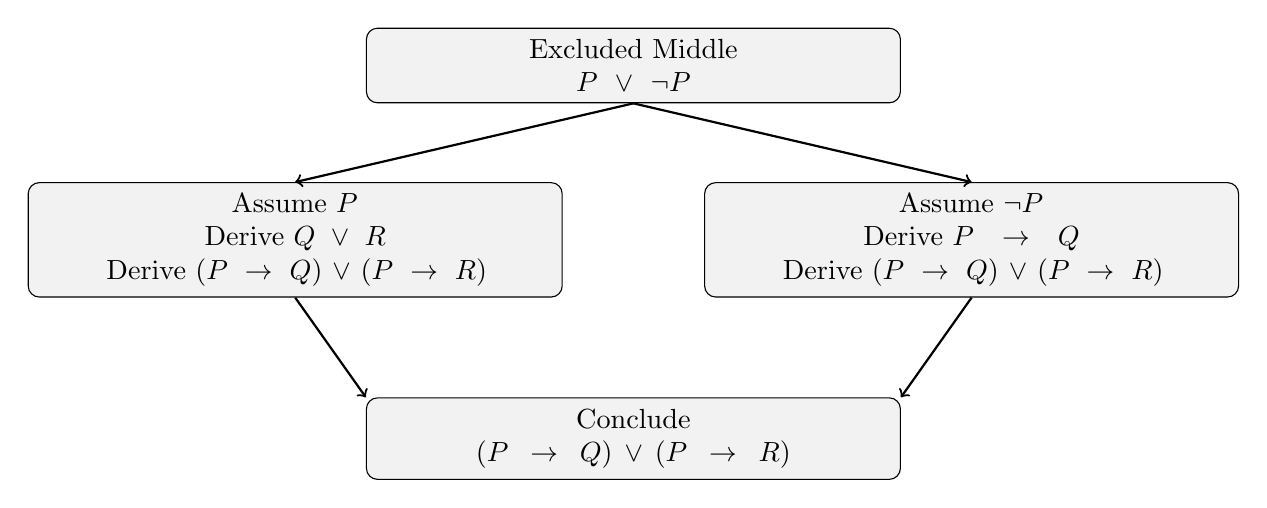
\begin{tikzpicture}[
  node distance=1.0cm and 0.3cm,
  box/.style={draw, rounded corners, fill=gray!10, inner sep=4pt, text width=6.5cm, align=center},
  arrow/.style={->, thick}
]

% Premise
\node[box] (prem) {Excluded Middle \\ $P\vee \neg P$};

% Subproofs side by side
\node[box, below left=1cm and -2.5cm of prem] (left) {
  Assume $P$ \\
  Derive $Q\vee R$ \\
  Derive $(P\to Q)\vee (P\to R)$
};
\node[box, below right=1cm and -2.5cm of prem] (right) {
  Assume $\neg P$ \\
  Derive $P\to Q$ \\
  Derive $(P\to Q)\vee (P\to R)$
};

% Conclusion directly beneath both
% \node[box, below=of $(left)!0.5!(right)$] (concl) {$R$};
\node[box, below=2cm of $(left)!0.5!(right)$] (concl) {Conclude \\
  $(P\to Q)\vee (P\to R)$};

% Arrows
\draw[arrow] (prem.south) -- (left.north);
\draw[arrow] (prem.south) -- (right.north);
\draw[arrow] (left.south) -- (concl.north west);
\draw[arrow] (right.south) -- (concl.north east);

\end{tikzpicture}
\end{frame} 


\begin{frame}

  \bigskip
  \begin{tabular}{>{\raggedleft\arraybackslash}p{1.5cm} >{\centering\arraybackslash}p{1.0cm} p{5cm} >{\raggedright\arraybackslash}p{3.5cm}}
1 & (1) & $(\mathit{P} \to \mathit{Q}) \to \mathit{P}$ & A \\
2 & (2) & $\neg \mathit{P}$ & A \\
3 & (3) & $\mathit{P}$ & A \\
2,3 & (4) & $\mathit{P} \wedge \neg \mathit{P}$ & 2,3 $\wedge$I \\
5 & (5) & $\neg \mathit{Q}$ & A \\
2,3 & (6) & $\neg \neg \mathit{Q}$ & 5,4 RA \\
2,3 & (7) & $\mathit{Q}$ & 6 DN \\
2 & (8) & $\mathit{P} \to \mathit{Q}$ & 3,7 CP \\
1,2 & (9) & $\mathit{P}$ & 1,8 MP \\
1,2 & (10) & $\mathit{P} \wedge \neg \mathit{P}$ & 9,2 $\wedge$I \\
1 & (11) & $\neg \neg \mathit{P}$ & 2,10 RA \\
1 & (12) & $\mathit{P}$ & 11 DN \\
$\varnothing$ & (13) & $((\mathit{P} \to \mathit{Q}) \to \mathit{P}) \to \mathit{P}$ & 1,12 CP \\
\end{tabular}


\end{frame}


\begin{frame}{Summary}

  \begin{itemize}
  \item With RA, we have completed the set of inference rules for
    propositional logic.
  \item These rules are provably \textbf{sound}: they do not permit a
    proof of something that has a truth-table counterexample.
  \item These rules are provably \textbf{complete}: anything
    semantically valid can be proven.
  \end{itemize}

\end{frame}  


  \section{Supplemental material}

  % --- Redundancies ---
\begin{frame}{Redundancies in Our System}
\begin{itemize}
  \item With RA, Modus Tollens (MT) and DN-Intro can be eliminated.
  \item Example: simulate MT using RA.
\end{itemize}

{\footnotesize
\begin{tabular}{>{\raggedleft\arraybackslash}p{1.5cm}
                >{\centering\arraybackslash}p{1.0cm}
                p{5cm}
                >{\raggedright\arraybackslash}p{3.5cm}}
1 & (1) & $P\to Q$ & A \\
2 & (2) & $\neg Q$ & A \\
3 & (3) & $P$ & A \\
1,3 & (4) & $Q$ & 1,3 MP \\
1,2,3 & (5) & $Q\wedge \neg Q$ & 4,2 $\wedge$I \\
1,2 & (6) & $\neg P$ & 3,5 RA \\
\end{tabular}
}
\end{frame}

\begin{frame}{Simulating DN-Intro}

\begin{tabular}{>{\raggedleft\arraybackslash}p{1.5cm}
                >{\centering\arraybackslash}p{1.0cm}
                p{5cm}
                >{\raggedright\arraybackslash}p{3.5cm}}
1 & (1) & $P$ & A \\
2 & (2) & $\neg P$ & A \\
1,2 & (3) & $P\wedge \neg P$ & 1,2 $\wedge$I \\
1 & (4) & $\neg\neg P$ & 2,3 RA \\
\end{tabular}

\end{frame}

\begin{frame}{Without RA}
RA itself can be simulated with other rules.  

Suppose $\Gamma, P \vdash Q\wedge \neg Q$. Then:
\begin{itemize}
  \item $\Gamma\vdash P\to Q$ and $\Gamma\vdash P\to \neg Q$.  
  \item By contraposition: $\Gamma\vdash \neg Q\to \neg P$.  
  \item Hence $\Gamma\vdash P\to \neg P$.  
  \item But $P\to \neg P \vdash \neg P$.  
\end{itemize}

So $\Gamma\vdash \neg P$.  
Still, RA feels more natural and symmetric.
\end{frame}

% --- Long proofs ---
\begin{frame}{More difficult proofs}
To show: $\vdash \:(P\to Q)\vee (Q\to P)$

\medskip \begin{itemize}
\item Strategy 1: Assume $\neg((P\to Q)\vee(Q\to P))$. Use DM to get
  $\neg (P\to Q)$ and $\neg (Q\to P)$. The former entails $P$ while
  the latter entails $\neg P$.
\item Strategy 2: Derive $Q\vee \neg Q$, then argue by cases using
  positive paradox and negative paradox in turn.
\end{itemize}
\end{frame}





\end{document}
%%% Local Variables:
%%% mode: latex
%%% TeX-master: t
%%% End:
